\section{Solução mecânica}
%TODO Estevão: solução final, detalhada  da mecanica com possiveis simulações

A solução de revestimento de uma pá de turbina \textit{in situ} requer um robô
de pequeno a médio porte, capaz de passar pelo limitado acesso da turbina. 
No entanto, a pá da turbina é uma peça com uma grande área a ser coberta pelo
revestimento sendo o robô incapaz de alcançar, de uma só posição, toda a sua
extensão. Assim, é necessário prover ao robô liberdade de posicionamento
para realizar o revestimento em uma pequena região da pá, por posição de
base.

Devido ao peso do manipulador e por questões de segurança, a movimentação deste
no interior da turbina não pode ser uma tarefa manual. Logo, uma base mecânica
deve ser capaz de levar o robô desde a escotilha até a posição ideal
para o revestimento, de forma segura e precisa. O dimensionamento desta base deve levar
em consideração todos os esforços de operação, como: o peso do sistema, as
cargas dinâmicas de movimentação do robô e o empuxo da pistola. 

Foram estudados diversos conceitos para os graus de liberdade providos pela
base mecânica. O estudo destes conceitos estão detalhados no artigo 
~\ref{EMMA_DETAIL}.

\subsection{Conceito}

A escolha do conceito da solução foi baseado nos graus de liberdade da base
mecânica para permitir ao robô movimentação e alcance necessários para realizar 
o revestimento. 

O conceito aqui aprofundado é denominado P-R-P-P, ou
Prismático-Rotacional-Prismático-Prismático.
A seguir estão descritas cada junta que compõe a base.

$\bullet$\textit{Prismática 1:} A primeira junta prismática é formada por um
trilho, sobre uma estrutura modular. Este trilho é denominado ''trilho primário'' e está
paralelo ao eixo da turbina, indo desde a escotilha de entrada até a região 
posterior da pá, próxima ao distribuidor.

$\bullet$\textit{Rotacional:} A segunda junta, rotacional, é formada por um
eixo apoiado sobre mancais de rolamento, que liga os trilhos ''primário'' e ''secundário''. 

$\bullet$\textit{Prismática 2:} A terceira junta,
prismática, é formada por um trilho, denominado ''trilho secundário'', também
sobre uma estrutura modular. Este trilho é posicionado paralelo ao plano
transversal da pá, e permitirá ao robô os deslocamentos laterais ao longo de toda a
extensão da largura da pá. 

$\bullet$\textit{Prismática 3:} A última junta, prismática, é formada por um
macaco mecânico tipo sanfona, com curso mínimo de $200~mm$, permitindo ao robô
maior alcance em altura.

A figura ~\ref{fig::conceito} apresenta o conceito descrito.

\begin{figure}[H]
	\centering
	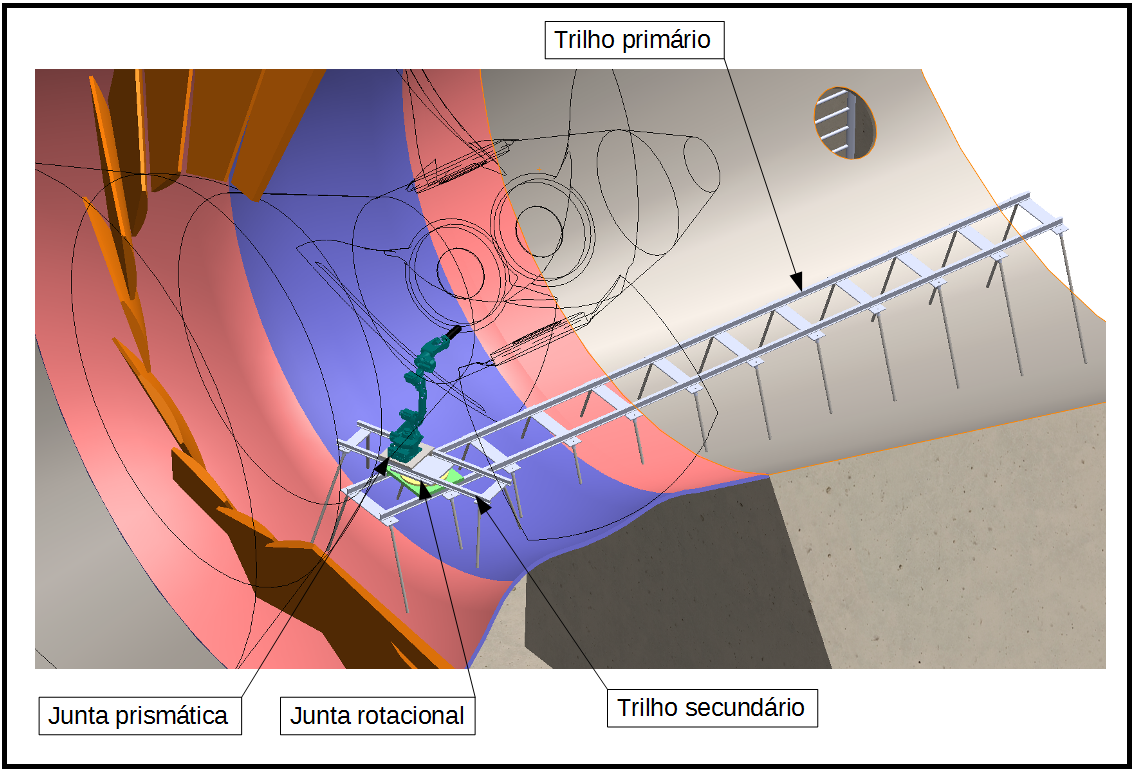
\includegraphics[width=0.9\columnwidth]{figs/conceito/conceito_P-R-P-P_01_tags}
	\caption{Conceito P-R-P-P da base mecânica}
    \label{fig::conceito}
\end{figure}

Neste conceito, o manipulador é movimentado pelo trilho primário até a região
próxima a pá. Em seguida é montado o trilho secundário a partir da base onde o
manipulador está fixado. A orientação do trilho secundário é definida pela
movimentação da junta rotacional entre os trilhos primário e secundário. A
partir daí, o manipulador pode ser movimentado ao longo do trilho secundário e
posicionado para o revestimento. Para as regiões de difícil alcance será
utilizada a junta de elevação.

\subsection{Constução}

\subsubsection{Trilho e carrinho}

Para movimentação e posicionamento precisos do manipulador foi selecionado o
sistema de trilho e carrinho de rolamento de esferas recirculantes. 
O trilho selecionado tem o perfil segundo a norma ISO 12090-1 e o carrinho segue
a norma DIN 645-1. 
Estes componentes são próprios para aplicações onde se requer grande capacidade
de carga e precisão de posicionamento.

\begin{figure}[H]
	\centering
	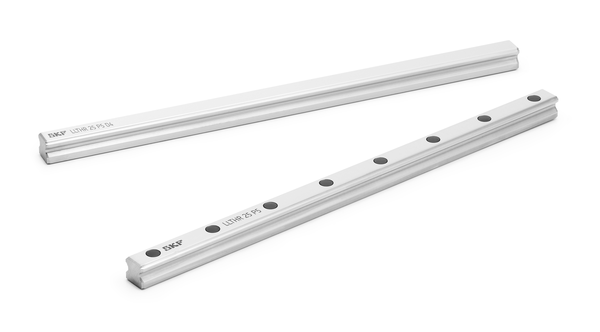
\includegraphics[width=0.7\columnwidth]{figs/construcao/trilho_LLT}
	\caption{Trilho para movimento linear}
    \label{fig::trilho}
\end{figure}

\begin{figure}[H]
	\centering
	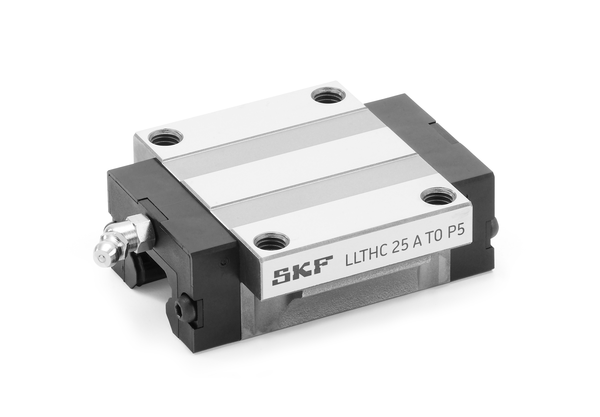
\includegraphics[width=0.7\columnwidth]{figs/construcao/carrinho}
	\caption{Carrinho de esferas recirculantes}
    \label{fig::carrinho}
\end{figure}

Estes componentes permitem algumas opções de montagens que variam de acordo com
a aplicação. 
Estas opções vão desde a utilização de um único trilho e único carrinho,
montagens com 1 trilho e 2 carrinhos, até montagens com 2 trilhos e 4 carrinhos,
mostrado na figura~\ref{fig::sist_2por4}.

\begin{figure}[H]
	\centering
	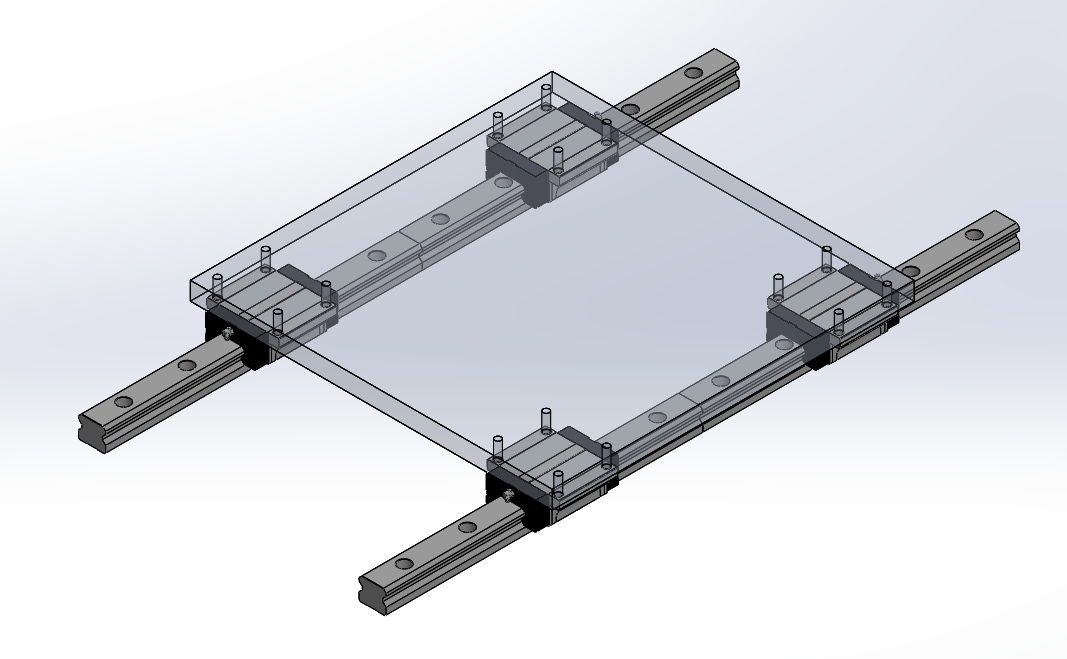
\includegraphics[width=0.9\columnwidth]{figs/construcao/sist_2por4}
	\caption{Montagem com 2 trilhos e 4 carrinhos}
    \label{fig::sist_2por4}
\end{figure}

As cargas promovidas pelo manipulador podem ser elevadas, sobretudo na base, que
reage às cargas distantes do ponto de fixação, causando momentos elevados. 
A vantagem da utilização de mais de um carrinho por trilho é a possibilidade de
anular-se os momentos de reação nos carrinhos, na direção ortogonal ao eixo do
trilho. 
No nosso caso, as cargas são variáveis em sua magnitude e direção.
Por esta razão, a configuração que utiliza 2 trilhos e 4 carrinhos é a mais
indicada, já que os carrinhos ficam livres de reagirem a momentos e as cargas ficam
dividas em mais componentes.

%TODO Estevão: incluir figura 4 carrinhos e 2 trilhos

%---------------------------------------------------------------------
\subsubsection{Perfil de alumínio estrutural} \label{sec::perfil}

A estrutura que servirá de base para o trilho deve ter como prinicipal
característica a modularidade. Devido à geometria variável do ambiente no
interior da turbina, é necessário também que esta estrutura permita 
flexibilidade de montagem dos apoios e ancoragens ao longo do trilho.
Cada módulo que da estrutura será composto pelo perfil estrutural onde
serão fixados o trilho e os acessórios de apoio e ancoragem da estrutura no
ambiente.
Tais módulos devem permitir transporte e montagem manuais, de forma fácil e
rápida.
Por isso, optou-se pelo perfil de alumínio estrutural. Este perfil possui
ranhuras para fixação de componentes padronizados que permite a construção
de uma grande variedade de estruturas funcionais de geometrias simples ou
complexas.

\begin{figure}[H]
	\centering
	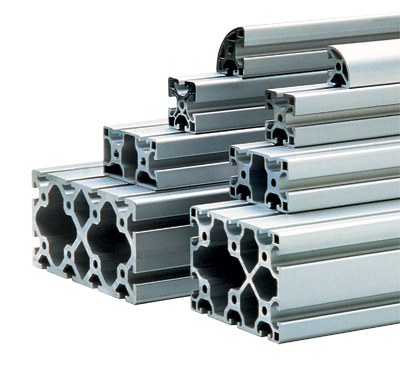
\includegraphics[width=0.7\columnwidth]{figs/construcao/aluminio_estrutural}
	\caption{Perfis de alumínio estrutural}
    \label{fig::aluminio_estrutural}
\end{figure}

A figura~\ref{fig::modulo_primario} apresenta um exemplo de um dos módulos do
trilho primário, a partir da montagem deste no perfil de alumínio
estrutural. Este módulo pode ser repetido ao longo do eixo longitudinal do
trilho, formando assim a estrutura completa do trilho. 
Para se ajustar ao ambiente da turbina, há variação apenas do comprimento dos
pés de apoio e dos braços de ancoragem, mantendo-se as mesmas dimensões de todos
os outros componentes.

\begin{figure}[H]
	\centering
	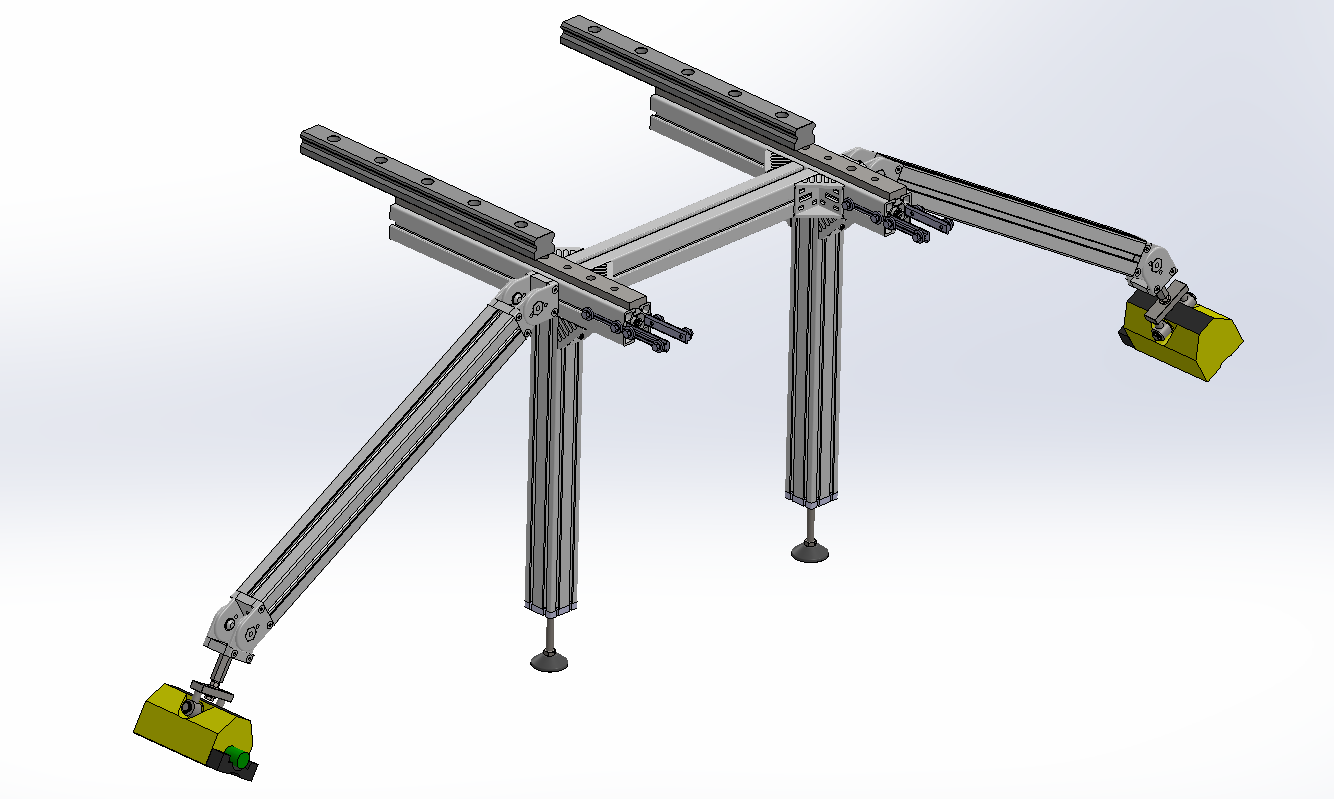
\includegraphics[width=0.9\columnwidth]{figs/construcao/modulo_primario}
	\caption{Perfis de alumínio estrutural}
    \label{fig::modulo_primario}
\end{figure}

%---------------------------------------------------------------------
\subsubsection{Pés de apoio}

Os pés de apoio da estrutura primária têm o objetivo de nivelar o trilho no
ambiente, permitindo que a estrutura possa formar um plano horizontal e paralelo
ao eixo da turbina. Devido às inclinações da superfície do túnel e do
aro-câmara, os pés de apoio devem permitir graus de liberdade que compensem
algum desvio. Além disto, o comprimento de cada ''perna'' da base varia ao
longo da estrutura, sendo necessário permitir uma margem de erro de
montagem a partir de uma regulagem de seu comprimento.

Foi verificado que o maior ângulo formado entre o eixo horizontal
e a superfície da turbina é de aproximadamente $9º$. Optou-se portanto por pés com
interface do tipo rótula, figura~\ref{fig::spindle}, que permitem até $10º$ de
inclinação entre a haste e à base, além de $75~mm$ de regulagem do
comprimento, pela rosca da haste.

\begin{figure}[H]
	\centering
	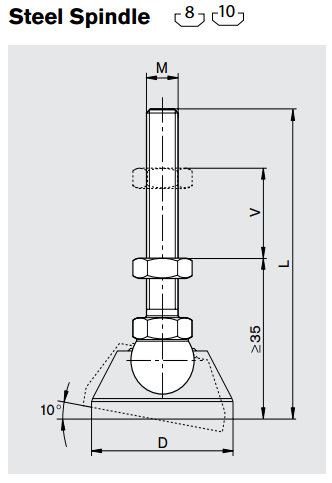
\includegraphics[width=0.4\columnwidth]{figs/construcao/spindle}
	\caption{Pé com interface rotular entre a haste e a base}
    \label{fig::spindle}
\end{figure}

%---------------------------------------------------------------------
\subsubsection{Ancoragem}

A ancoragem da estrutura é importante para prevenir movimento da base quando o
robô estiver em movimento. Sua principal função é tornar a base rígida o
suficiente para que as deformações elásticas e vibrações da estrutura não
interfiram na precisão do processo de revestimento.

Os braços de ancoragem são constituídos de duas juntas rotacionais em cada
extremidade. Estas juntas permitem que o braço se ajuste a superfície da
turbina, posicionando as bases magnéticas na orientação ideal para o acoplamento
magnético mais eficiente possível. A figura~\ref{fig::ancoragem} apresenta um
dos braços de ancoragem.

\begin{figure}[H]
	\centering
	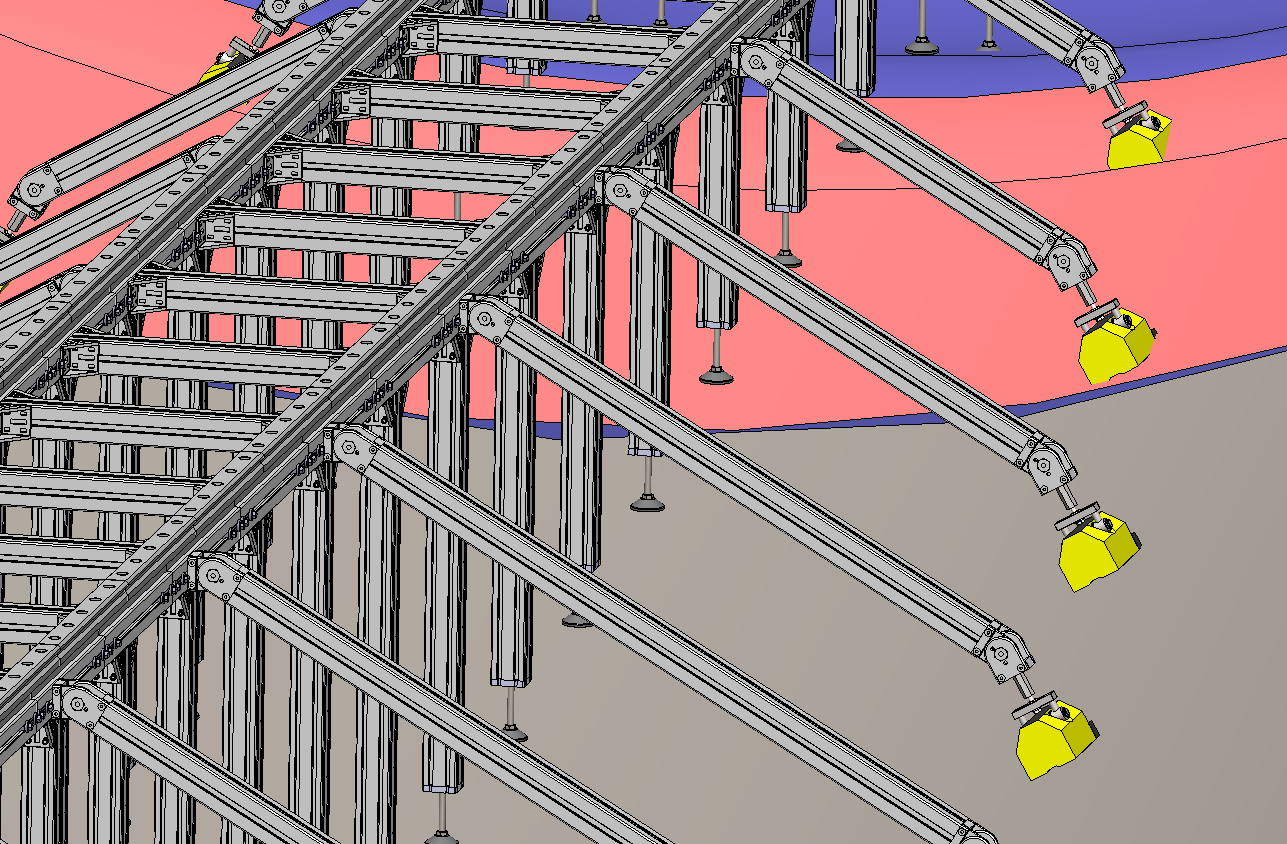
\includegraphics[width=0.9\columnwidth]{figs/construcao/ancoragem}
	\caption{Braços de ancoragem do trilho primário}
    \label{fig::ancoragem}
\end{figure}

%---------------------------------------------------------------------
\subsubsection{Bases magnéticas}

As bases magnéticas são os elementos de fixação não-permanentes que serão
utilizados para ancoragem da estrutura no ambiente da turbina. Foram realizados
testes para verificação da carga máxima suportada e o resultado foi
satisfatório e apresentado no anexo do relatório %\cit[emma-detail].

As bases magnéticas são equipamentos comerciais cuja principal aplicação na
indústria é o içamento e movimentação de peças metálicas. Este equipamento é
composto por imãs permanentes que são alinhados através de uma alavanca em sua
carcaça. Desta forma, é possível ''ligar'' e ''desligar'' o imã a qualquer
momento.

\begin{figure}[H]
	\centering
	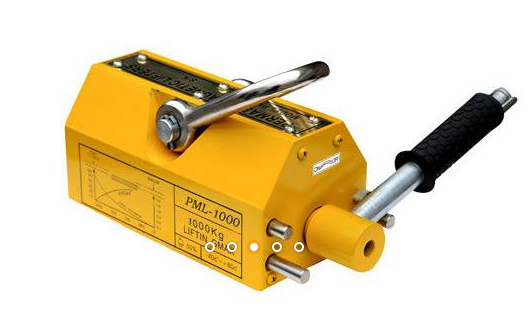
\includegraphics[width=0.5\columnwidth]{figs/construcao/base_magnetica}
	\caption{Base magnética para ancoragem}
    \label{fig::base_magnetica}
\end{figure}

%---------------------------------------------------------------------
\subsubsection{Junta de rotação}

%---------------------------------------------------------------------
\subsubsection{Junta de elevação}

%---------------------------------------------------------------------
\subsubsection{Montagem}

A montagem da base mecânica no interior da turbina é feita a partir de módulos
(submontagens que formam elementos básicos de uma montagem maior). O exemplo de
um módulo da estrutura primária foi apresentado na
figura~\ref{fig::modulo_primario}, na seção~\ref{sec::perfil}. 

Neste conceito, primeiro monta-se a estrutura e trilho
primários, e então, monta-se a base do robô no trilho primário. Esta base contém
os elementos que permitem os graus de liberdade de rotação e prismático
(elevação) e também serve de origem para a montagem da estrutura e trilho
secundários. 

\begin{figure}[H]
	\centering
	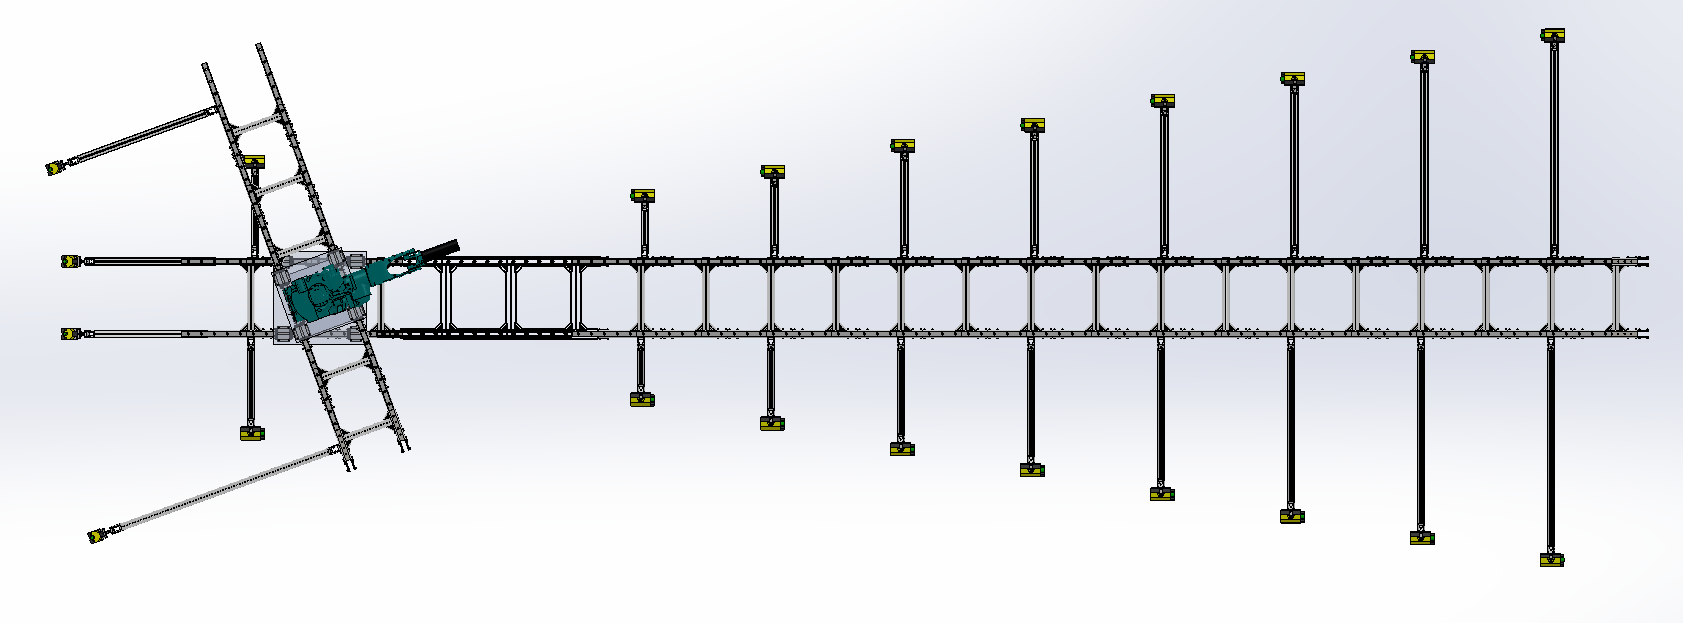
\includegraphics[width=0.9\columnwidth]{figs/construcao/EMMA_Base_Secundaria_04}
	\caption{Montagem da base mecânica}
    \label{fig::EMMA_Base_Secundaria_04}
\end{figure}

A figura~\ref{fig::EMMA_Base_Secundaria_04} apresenta uma vista superior da
montagem da base mecânica e a figura~\ref{fig::EMMA_Base_Secundaria_01}
apresenta a montagem no interior da turbina, em uma configuração de operação na
face posterior da pá. Nota-se que é necessária a desmontagem de parte do trilho
primário para posicionar a pá no melhor ângulo em relação à base. Esta é mais
uma vantagem de se ter um conceito modular para a estrutura.

\begin{figure}[H]
	\centering
	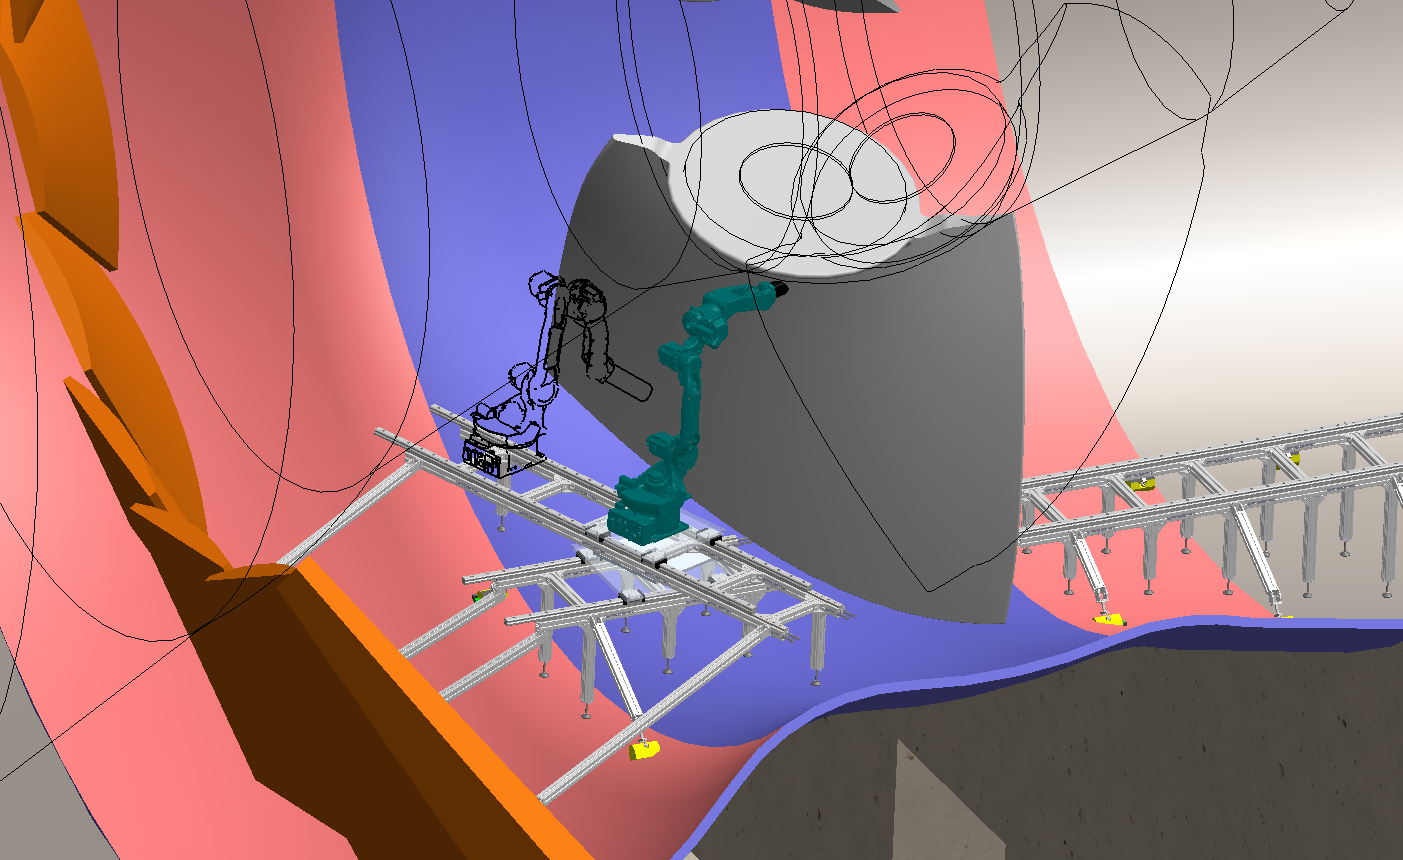
\includegraphics[width=0.9\columnwidth]{figs/construcao/EMMA_Base_Secundaria_01}
	\caption{Montagem da base mecânica no interior da turbina}
    \label{fig::EMMA_Base_Secundaria_01}
\end{figure}

